\section{Inverse Language Modeling}

\begin{frame}{Attacking LLMs with GCG}
\note{
    GCG finds attack sequences $\bxa$ such that they can link better to a given continuation $\by$, \\
    starting from a random one-hot sequence of tokens and \\
    iteratively optimize it using \textbf{gradient} information. \\
    This table must be read: $\bx || \by$ and $\bxa || \by$. \\
    These sequences are called \emph{Evil Twins} in the Prompts have evil twins paper. \\
    --------- \\
    OUR GOAL? Prevent their existence, or limit the success rate of this attack.
}
    Greedy Coordinate Gradient is an algorithm to find a sequence of tokens $\bxa$ such that the LLM will complete with $\by$ that we want --- using \highlight{gradients} on input tokens
    \vfill

    \begin{table}[]
    \centering
    \resizebox{\textwidth}{!}{
        \begin{tabular}{llc}\toprule
        \textbf{Input} & \textbf{Output $\by$} & \textbf{Loss} \\
        \midrule
        %\cline{2-3}
        $\bx$~: Stevens recorded and produced the album at multiple & \multirow{2}{*}{locations in the United}  & 5.3642 \\
        $\bxa$: Zo Certified Cities (. broadcastquartered Fitness Academy thirteen   & &  \textbf{5.1302} \\
        \midrule
        $\bx$~: After the introduction of the Majors , The   & \multirow{2}{*}{British Army was divided}   & 11.2146 \\
        $\bxa$: REQU Apart British received reformsMilitaryestic Division The  & &  \textbf{7.1899} \\
        \midrule
        $\bx$~: The founding director , Peggy Loar , left   & \multirow{2}{*}{the University of California}   & 7.2669\\
        $\bxa$: tested UberERIC definitionCalifornia sustainability RutgersOL Jensen regarding  & &  \textbf{6.4402} \\
        \midrule
        $\bx$~: Ruiz notes that writing also has the power & \multirow{2}{*}{\centering to change the world} & 5.9135 \\
        $\bxa$: Report Global feminism agenda Representatives tell Sacredixties Trying & & \textbf{4.6041} \\
        \bottomrule
        \end{tabular}
    }
    \caption{They are called "Evil Twins"}
    \end{table}
\end{frame}

\begin{frame}{Difficulties of LLMs}
    What about LLMs?

    \begin{itemize}
        \item Input is \highlight{sequential}
        \note{$\rightarrow$ a single token cannot determine what's the next token to predict}
        \item The same sequence can continue in multiple ways $\rightarrow$ \highlight{multiple} valid classes
        \item The input space is \highlight{discrete} ($|\mathcal{V}|$)
    \end{itemize}
\end{frame}

\begin{frame}{Introducing ILM}
\note{
    At this point, we can introduce Inverse Language Modeling. \\
    \textbf{GOAL}: train LLMs, or fine-tune them, such that they internally "understand" what they are conditioned on. \\
    This is somehow based on the idea of LLMs as stochastic parrots. \\
    \textbf{KEY IDEAS}: create a new training procedure that makes them \textbf{grounded} to the input, exploiting weights.
}
    \begin{itemize}
        \item \highlight{Goal:} train LLMs to both generate text and \emph{understand what they are conditioned on} 
        \underline{\textbf{(inversion)}}
        from the output
        \item \highlight{Key Ideas:}
            \begin{itemize}
                \item Create a new training procedure that adds more \underline{\textbf{robustness}} in the loop
                \item Reconstruct input from the output, using $\nabla_\bx \loss$
            \end{itemize}
    \end{itemize}
\end{frame}

\begin{frame}{Introducing ILM}
\note{
    This illustration graphically shows the logic: \\
    - originally, they go from left to right \\
    - but it can also go from right to left, using gradients information.
}
    \begin{figure}
    \centering
    \vspace{0.5cm}
    \begin{overpic}[width=0.7\linewidth]{assets/forward_backward_llm}
        \put(5.5,0){$\bx_1$}\put(19.5,0){$\bx_2$}\put(33.5,0){$\bx_3$}
        \put(5.5,27){$\bx_2$}\put(19.5,34){$\bx_3$}\put(33.5,44){$\bx_4$}
        \put(60,43.5){$\bx_2$}\put(72,43.5){$\bx_3$}\put(87,43.5){$\bx_4$}
        \put(60,0){$\bx_1$}\put(72,10){$\bx_2$}\put(87,18){$\bx_3$}
        \put(17,59.5){{\footnotesize \textbf{Now}}}
        \put(68,59.5){{\footnotesize \highlight{Proposed}}}
        \put(0,55){{\footnotesize Autoregressive forward}}
        \put(55,55){{\footnotesize Autoregressive backward}}
        \put(5,49){{\scriptsize $p(\bx_i|\bx_1,\ldots,\bx_{i-1})$}}
        \put(50,49){{\scriptsize$p\big(\bx_{i-1}| \nabla_{\bx_{i-1}}p(\bx_i|\bx_1,\ldots,\bx_{i-1})\big)$}}
    \end{overpic}
    \end{figure}
\end{frame}

\begin{frame}{ILM Inversion Procedure}
\note{
    Let's make an example: \\
    We have a sentence, like \emph{The pen is on the table} \\
    It gets split: \\
    - prefix: \emph{the pen is} \\
    - suffix: \emph{on the table} \\
    . \\
    Here, we have the suffix and predict backward the prefix.
}
    \centering
    Split it into the original prefix $\bx_p = \bx_{0:k}$ and the suffix $\bx_s = \bx_{k:n}$ \\
    \vfill
    $\bx =$ The pen is on the table \\
    \vspace{0.5cm}
    \hfill $\bx_p =$ \highlight{The pen is} \hfill $\bx_s = $ on the table \hfill $\;$\\
\end{frame}

% \begin{frame}{Gradients Received by the Tokens}
% \note{
%     But how is that possible? What's the \textbf{theoretical} rationale behind it? \\
%     From this diagram, you can see that if we change a token in the middle, like $\be_3$, \\
%     it influences the hidden states only in the future, \\
%     but gradients carry out the information of the overall sentence, \\
%     since the gradients of the previous tokens (the \textbf{past}) change as well.
% }
%     Gradients received on a single token embedding,
%     carry information of the whole sentence

%     \begin{figure}
%         \centering
%         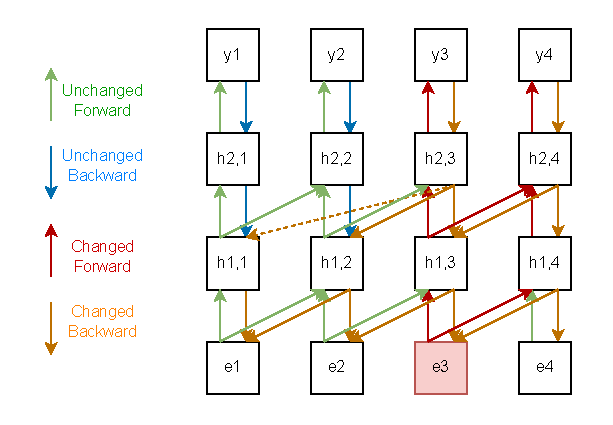
\includegraphics[height=0.6\paperheight]{assets/llm_gradients_changing_embedding.drawio.pdf}
%     \end{figure}
% \end{frame}

\begin{frame}{Gradients Received by the Tokens}
\note{
    This sentence well describes the rationale.
}
    \begin{quote}
        \centering
        A causal model looks ahead, \\ but only its gradients disclose the pasts that might have built that future.
    \end{quote}
\end{frame}

\begin{frame}{ILM Training Procedure}
    
\includegraphics[width=\linewidth]{assets/grad_lm_head_parallelism_0.drawio.pdf}
    \vspace{1.5cm}
    
    \centering
    Given the input sentence $\bx_0, \bx_1, \bx_2, \dots, \bx_{n-1}$
\end{frame}

\begin{frame}[noframenumbering]{ILM Training Procedure}
    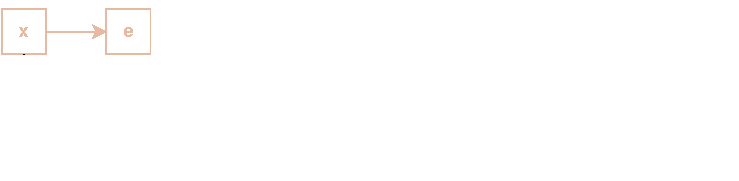
\includegraphics[width=\linewidth]{assets/grad_lm_head_parallelism_1.drawio.pdf}
    \vspace{1.5cm}
    
    \centering
    Embed the input sentence tokens into $\be_0, \be_1, \be_2, \dots, \be_{n-1}$
\end{frame}

\begin{frame}[noframenumbering]{ILM Training Procedure}
    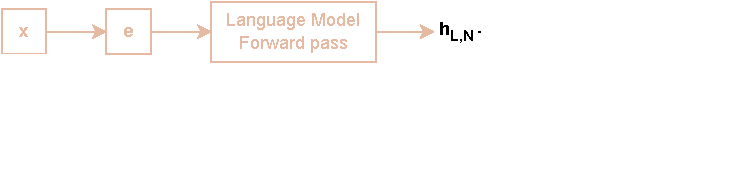
\includegraphics[width=\linewidth]{assets/grad_lm_head_parallelism_2.drawio.pdf}
    \vspace{1.5cm}
    
    \centering
    Pass through the Transformer Decoder layer, up to the final hidden state $\bh_0, \bh_1, \bh_2, \dots, \bh_{n-1}$
\end{frame}

\begin{frame}[noframenumbering]{ILM Training Procedure}
    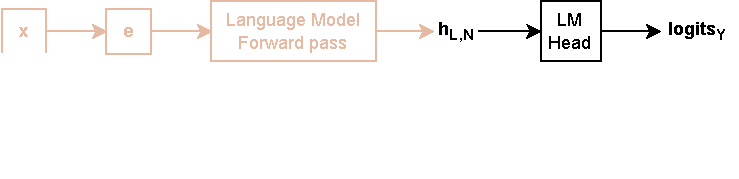
\includegraphics[width=\linewidth]{assets/grad_lm_head_parallelism_3.drawio.pdf}
    \vspace{1.5cm}
    
    \centering
    Using the Classifier Head, predict $\by_0, \by_1, \by_2, \dots, \by_{n-1}$
\end{frame}

\begin{frame}[noframenumbering]{ILM Training Procedure}
    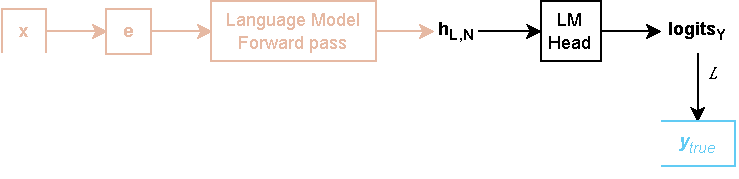
\includegraphics[width=\linewidth]{assets/grad_lm_head_parallelism_4.drawio.pdf}
    \vspace{1.5cm}
    
    \centering
    Compute the loss $\loss_{CE} = CE(\bx_{1:n}, \by_{0:n-1})$ comparing the predictions with the ground-truth
\end{frame}

\begin{frame}[noframenumbering]{ILM Training Procedure}
    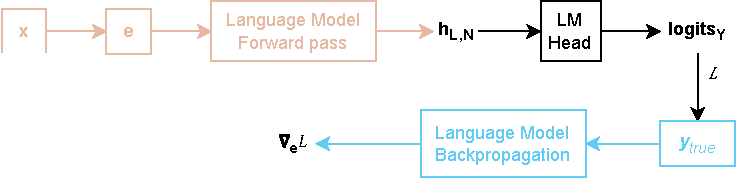
\includegraphics[width=\linewidth]{assets/grad_lm_head_parallelism_5.drawio.pdf}
    \vspace{1.5cm}
    
    \centering
    Backpropagation: compute the gradients $\nabla_{\be_{0:n-1}} \loss$
\end{frame}

\begin{frame}[noframenumbering]{ILM Training Procedure}
    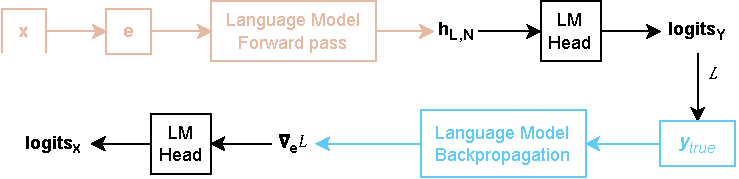
\includegraphics[width=\linewidth]{assets/grad_lm_head_parallelism_6.drawio.pdf}
    \vspace{1.5cm}
    
    \centering
    From the gradients, predict the input tokens $\bx_{0:n-1}$
    \note{Use the gradients as if they were the last hidden state and use them to predict the input $\bx$ tokens}
\end{frame}

\begin{frame}[noframenumbering]{Parallelism}
    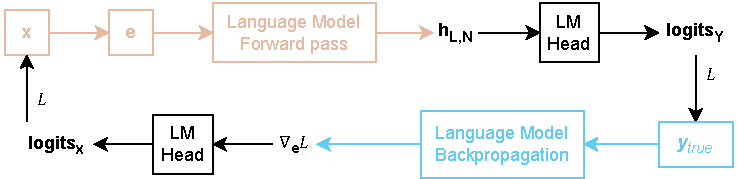
\includegraphics[width=\linewidth]{assets/grad_lm_head_parallelism.drawio.pdf}
    \vspace{1.5cm}
    
    \centering
    As if it were really \highlight{cyclic}! \\
    Parallelism between the last hidden state and the gradients on the embeddings
\end{frame}

\begin{frame}{More Parallelism: Weight Tying}
\note{
    In some LLMs, weight tying makes the LM Head projection and the Embeddings matrix to be exactly the same Tensor in memory!
}
    \centering
    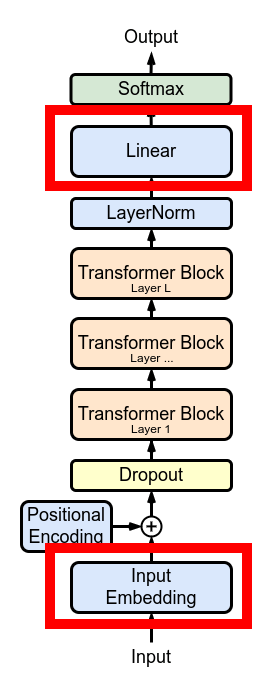
\includegraphics[height=0.8\paperheight]{assets/gpt_weight_tying.png}
\end{frame}



\begin{frame}{ILM Variants}
\note{
    We end up with this combined loss, both for Cross-Entropy forward and backward. \\
    This is implemented using PyTorch-supported \textbf{double Backpropagation}. \\
    --------- PAUSE --------- \\
    We have some variants: \\
    - identity, what we just said. It might hypothetically learn some identity function, as in AutoEncoders without a bottleneck \\
    - bert-like, imitating the BERT training procedure when going backward on the Gradients \\
    - inv-first, that just works on the very first token, splitting sentences. \\
    --------- PAUSE --------- \\
    Classification: \\
    - we can use these gradients as a pure value \\
    - or follow the natural definition of a gradient as a direction and go in its negative direction \\
}
    \begin{equation*}
    \loss =
    \underbrace{\loss_{CE}(\by_\text{true}, \by_\text{pred})}_\text{Forward: from the input x, encode y}
    +
    \underbrace{\lambda\ \loss_{CE}(\bx, f(\bx, \nabla\bx))}_\text{Backward: from gradients, decode back x}
    \end{equation*}

    \pause
    \begin{itemize}
        \item \highlight{Identity}: what we have discussed so far
        % \begin{itemize}
        %     \item $\nabla_\be \loss$ theoretically has access to $\bx$ $\rightarrow$    \textbf{possible shortcut}
        % \end{itemize}
        \pause
        \item \highlight{BERT-like}: masking the input tokens on the gradients
        \begin{itemize}
            \item When computing $\nabla_\be$, replace 10\% tokens to predict from the gradients with \texttt{[PAD]} \\ $\rightarrow$ it should understand what's missing
        \end{itemize}
        \pause
        \item \highlight{Inv-First}: assign the first token to \texttt{[PAD]} and invert it
    \end{itemize}
    
    \pause
    \vspace{0.5cm}
    \textbf{Classification Stategies:}
    \pause
    \begin{itemize}
        \item Use gradient as \highlight{value} --- $f(\nabla_{\bx_i}\loss_{CE})$
        \pause
        \item Use gradient as \highlight{direction} --- $f(\bx_i - \nabla_{\bx_i}\loss_{CE})$
    \end{itemize}
\end{frame}


% \begin{frame}{ILM Inversion Procedure}
%     \centering
%     From the gradients on the input, predict the previous token \emph{(one at a time)} \\
%     \vspace{1cm}
%     Do a \highlight{Beam Search}: keep the $b$ most probable prefixes, not just one
% \end{frame}


\begin{frame}{But we don't have billions of dollars}
\note{
    However, we trained LLMs, with lots of different variants to compare. \\
    We HAD to stay on a small example, to validate the idea, \\
    scaling it in a future time.
}
    These results have been obtained on a tiny LLM:
    \begin{itemize}
        \item Only 10M parameters
        \item A vocabulary of just 2048 tokens
        \item A simple corpus (\texttt{TinyStories} dataset)
    \end{itemize}

    \vfill
    It will be scaled to Llama-1B in the future.
\end{frame}
